\documentclass[a4paper, 11pt]{article}
\usepackage[british]{babel}
\usepackage{graphicx}
\usepackage[top=3cm, bottom=3cm, left = 2cm, right = 2cm]{geometry} 
\geometry{a4paper} 
\usepackage[utf8]{inputenc}
\usepackage[skip=2pt]{caption}

\begin{document}

\title{Intro to Machine Learning Coursework 1 Report - Decision Trees}

\author{Musawer Hussain, Vladimir Volgin, Oleg Tretieu}

\maketitle

\section{Introduction}
This is the final report of the first Introduction to Machine Learning coursework where we have implemented a decision tree algorithm and use it to determine one of the indoor locations based on WIFI signal strengths collected from a mobile phone. We were given two datasets, a clean dataset and noisy dataset and we have trained decision trees on each of them separately.
\\ \\
In this report we will first show the output of one of our decision trees formed, followed by listing out the evaluation metrics we have calculated for decision trees trained on both clean and noisy datasets before finally providing a short analysis of both the results and the difference in the two datasets.

\section{Image of the Decision Tree Formed}

The following is the Decision Tree that was formed as a result of doing 10-fold cross validation on the clean-dataset. This is the output of the visualisation function.

\begin{figure}[h]
  \centering
  \raisebox{0.0\height}{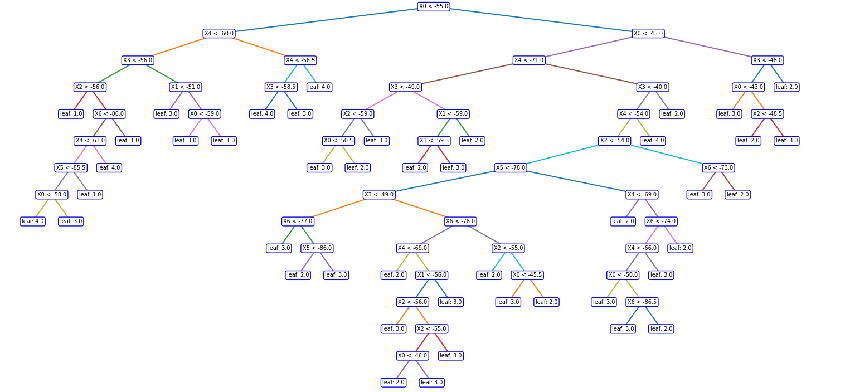
\includegraphics[width=14.2540994359176cm,height=6.58685884822248cm]{report-1.pdf}}
  \caption{Output of the decision tree visualisation function on the clean dataset.}
\end{figure}

\pagebreak
\section{Evaluation Metrics}

    \subsection{Clean data set}
    \renewcommand{\arraystretch}{2}
    \begin{table}[htb]
      \centering
      \caption{Confusion matrix for clean dataset} \
      \begin{tabular}{|l|l|l|l|l|}
      \hline
                    & Room 1 predicted & Room 2 predicted & Room 3 predicted & Room 4 predicted \\ \hline
      Room 1 actual & 496              & 0                & 2                & 2                \\ \hline
      Room 2 actual & 0                & 478              & 22               & 0                \\ \hline
      Room 3 actual & 1                & 18               & 479              & 2                \\ \hline
      Room 4 actual & 3                & 0                & 0                & 497              \\ \hline
      \end{tabular}
    \end{table}
    \textbf{%
    \begin{tabular}{l l}
        Average Accuracy: & 0.975 \\
        Recall: & \\
        & Room 1: 0.992 \\
        & Room 2: 0.956 \\
        & Room 3: 0.958 \\
        & Room 4:  0.994 \\
        Precision: & \\
        & Room 1: 0.992 \\
        & Room 2: 0.964 \\
        & Room 3: 0.952 \\
        & Room 4:  0.992 \\
        F1-measures: & \\
        & Room 1: 0.992 \\
        & Room 2: 0.960 \\
        & Room 3: 0.955 \\
        & Room 4: 0.993 \\
    \end{tabular}%
    }

    
    \subsection{Noisy data set}
    \renewcommand{\arraystretch}{2}  
    \begin{table}[htb]
      \centering
      \caption{Confusion matrix for noisy dataset}
      \begin{tabular}{|l|l|l|l|l|}
      \hline
                    & Room 1 predicted & Room 2 predicted & Room 3 predicted & Room 4 predicted \\ \hline
      Room 1 actual & 379              & 49               & 19               & 43               \\ \hline
      Room 2 actual & 29               & 398              & 47               & 23               \\ \hline
      Room 3 actual & 30               & 37               & 410              & 38               \\ \hline
      Room 4 actual & 47               & 30               & 37               & 384              \\ \hline
      \end{tabular}
    \end{table}
    \textbf{Accuracy:} 0.7855000000000001 \\
    \\
    \textbf{Recall:} \\
    Room 1: 0.77275535 \\
    Room 2: 0.80197697 \\
    Room 3: 0.79740095 \\
    Room 4: 0.77106065 \\
    \\
    \textbf{Precision:} \\
    Room 1: 0.78238612 \\
    Room 2: 0.77477728 \\
    Room 3: 0.79695117 \\
    Room 4: 0.78396774 \\
    \\
    \textbf{F1-measures:} \\
    Room 1: 0.7774359 \\
    Room 2: 0.78733927  \\
    Room 3: 0.79766537 \\
    Room 4: 0.77890467 \\
    
\pagebreak

\section{Analysis}

When using the clean data, the vast majority of the rooms are identified
correctly. We see from the confusion matrix that the rooms which were most
often confused with eachother are Room 2 and Room 3. With the noisy data,
while most rooms are still correctly recognised, there is a significant
amount of incorrect classifications. Most notably: Room 1 often gets misclassified as
Room 2, Room 4 as Room 1, and Room 2 as Room 3.
\

The performance on the noisy dataset is significantly worse than on the clean
dataset, which we can see by comparing the evaluation metrics above. This
could be caused by the decision tree overfitting when training on the noisy
data, effectively ``learning the noise'', which leads to worse generalisation.
Furthermore, the noisy dataset is slightly unbalanced, as Room 3 has 515
samples, whereas Room 1 only has 490, so it is necessary to look at the
normalized confusion matrix.


\end{document}

